%
% latex-sample.tex
%
% This LaTeX source file provides a template for a typical research paper.
%

%
% Use the standard article template.
%
\documentclass{article}

% The geometry package allows for easy page formatting.
\usepackage{geometry}
\geometry{letterpaper}

% Load up special logo commands.
\usepackage{doc}

% Package for formatting URLs.
\usepackage{url}

% Packages and definitions for graphics files.
\usepackage{graphicx}
\usepackage{epstopdf}
\DeclareGraphicsRule{.tif}{png}{.png}{`convert #1 `dirname #1`/`basename #1 .tif`.png}

%
% Set the title, author, and date.
%
\title{Dating Website Interfaces}
\author{Joseph Crawley}
\date{September 18, 2012}

%
% The document proper.
%
\begin{document}

% Add the title section.
\maketitle

% Add an abstract.
\abstract{}
For this assignment, Terran Moore and I looked how Match.com, Eharmony.com, and ChristianMingle.com measured in the usability metrics of Learnability, Satisfaction, and Efficiency. For this assignment, we had 5 users create profiles and complete similar tasks in order to measure these metrics.  

% Add various lists on new pages.
\pagebreak
\tableofcontents


%\listoffigures


%\listoftables

% Start the paper on a new page.
\pagebreak

%
% Body text.
%
\section{Learnability}
\label{Learnability}

\subsection{E-harmony.com}
Users were able to fill out profiles almost instantly. Searching was hard to understand and users became frustrated with the searching of the system.

\subsection{Match.com}
Menus were easy to understand and users could fill out profiles almost instantly. The searching function was easy to pick up on for users, and users could navigate the site with ease.

\subsection{ChristianMingle.com}
The site was very simple and easy to understand. Menus were clearly marked, and everything was labeled very quickly.


\section{Efficiency}
\subsection{E-harmony.com}
E-harmony was efficient on every test except for search ability, which it tested very poorly in. Its search ability was foreign to users who were familiar with networking sites and caused users to be frustrated.

\subsection{Match.com}
Match.com was very intuitive to users for all aspects. Users felt that they could navigate the site quickly and efficiently with little errors and with a low learning curve.

\subsection{ChristianMingle.com}
Users liked how simple ChristianMingle.com was. They felt that the simplicity helped them navigate the site easily. The only thing that was not simple was updating profile information, which took users a few more clicks than necessary.


\section{Satisfaction}
\subsection{E-harmony.com}
Users felt this site was very good for something, but bad for dating itself. Users felt that it was next to impossible and very timely to connect with matches. Users had low satisfaction with the site.


\subsection{Match.com}
	Users felt that this was the preferred choice in dating websites. It combined the comprehensiveness of E-harmony with the comprehensiveness of Match.com. Users were happy with how quick they picked up the site and how natural the interface was.

\subsection{ChristianMingle.com}
Users felt Christian Mingle was easy to use, but too simple. Users did not feel that the creating a profile interface was comprehensive enough. Although the menus were simple, they felt that the actions they wanted to take were not always available in the menus.

\section{Expectations of Dating Interfaces}

For our report, we could not find any specific reference or guide specific to dating websites, so we used the government usability guidelines. The below sections will contain excerpts from usability.gov, and how they are seen on the dating websites.

\subsection{"Designers should make every attempt to reduce the user’s workload by taking advantage of the computer’s capabilities."}
Since dating websites often require a lot of input when making a profile, dating websites should have efficient ways to enter data and also vary in data entry style so that the user does not become bored.

\subsubsection{E-harmony.com}
When filling out a profile on E-harmony, the user is asked a serious of personality questions. Almost all of the questions were in the formal as seen in Figure \ref{Eharm1}. The users in our tests often felt that they were bombarded with questions. The E-harmony questionnaire was the longest, therefore took our users the longest to fill out. Our users were frustrated with the amount of questions, and since most of the questions were in the same format, our users were bored and began to answer questions quickly and less efficiently. E-harmony could change the style of how they ask questions after every few responses.

\begin{figure}
\centering
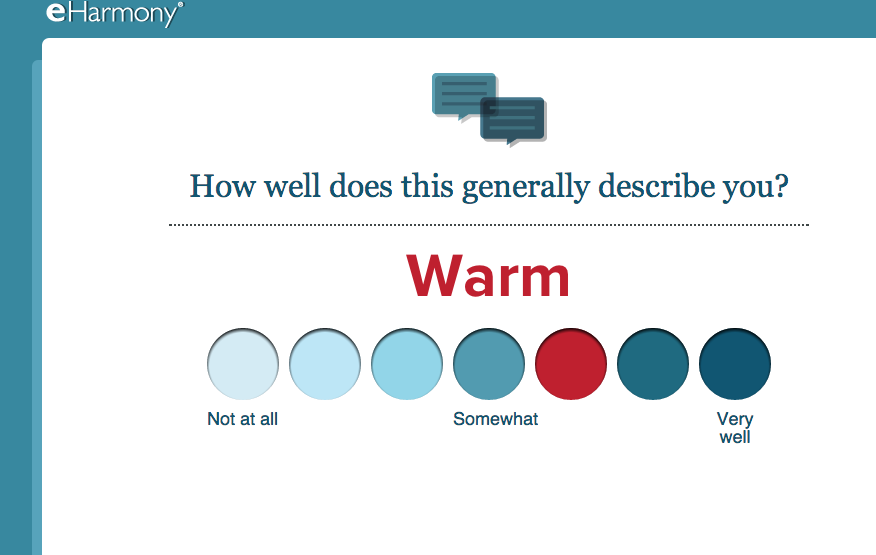
\includegraphics[width=4in]{Eharm1.png} 

\caption{E-Harmony personality questions}
\label{Eharm1}
\end{figure}

\subsubsection{Match.com}
Match.com does a good job of asking question multiple ways. Like Figure \ref{Match1}, there are 4-7 questions on a page, and there are multiple ways to submit input on this page. This kept users on their toes and stopped users from blindly answering questions. The only drawback to this interface is that the users spent more time per question than they did with E-Harmony. Users had to adjust answering in different ways, which made the questionnaire take more time.  

\begin{figure}
\centering
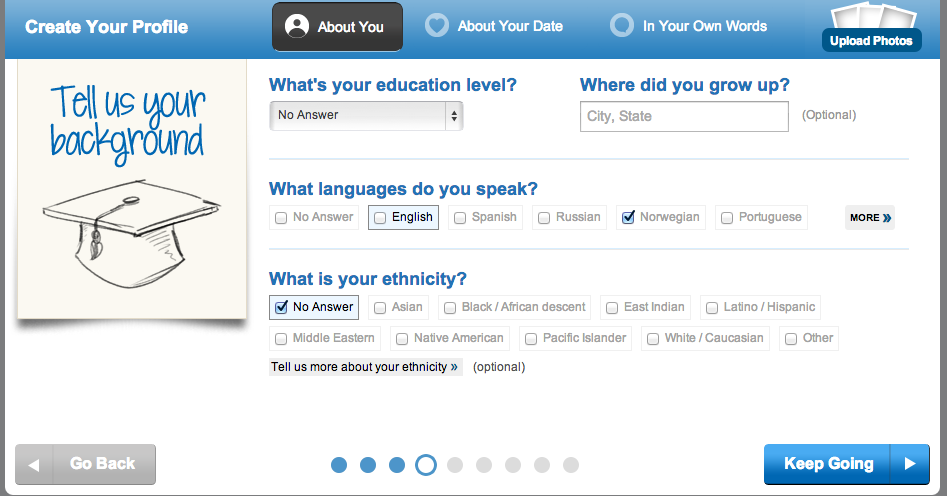
\includegraphics[width=4in]{Match1.png} 

\caption{Match.com personality questions}
\label{Match1}
\end{figure}

\begin{figure}
\centering
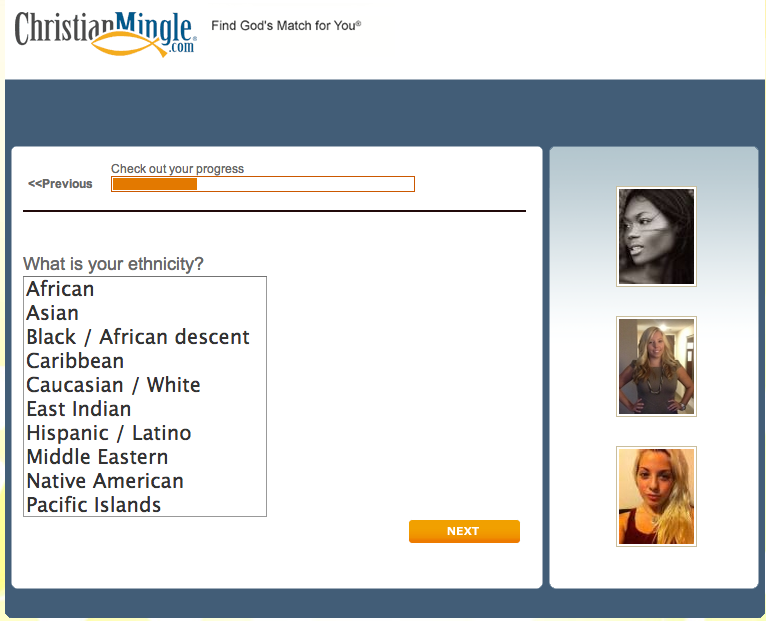
\includegraphics[width=4in]{CM1.png} 

\caption{ChristianMingle.com personality question page}
\label{CM1}
\end{figure}

\subsubsection{ChristianMingle.com}
Just like E-Harmony, Christian Mingle only used one type of input submission for its questions. However, Christian Mingle had a lot fewer questions than E-Harmony, so the user never had the opportunity to be bored by reading questions. The only concern with the question form was that there was no way to change answers if mistakes were made. Besides that, questions were easy to answer and process.



\subsection{“Results of user searches provide the precise information being sought, and in a format that matches users’ expectations.”}
On dating websites, searching for people or matches is extremely important. For this test, we asked users to find a 29 year-old Asian woman in St.Louis. We observed how users in this test could navigate the search function, and this is what we found.

\begin{table}
\caption{Sidebar searches for three dating websites}
\centering
\begin{tabular}{|c|c|c|}\hline
E-harmony & Match.com & Christian Mingle \\\hline\hline\hline
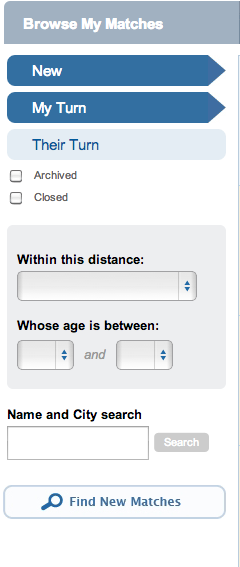
\includegraphics[width = 2in]{Eharm2.png} & 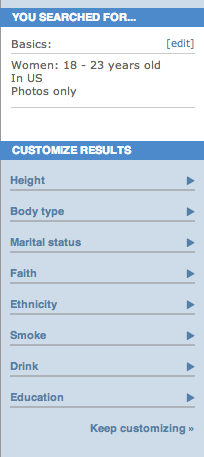
\includegraphics[width = 2in]{Match2.png} & 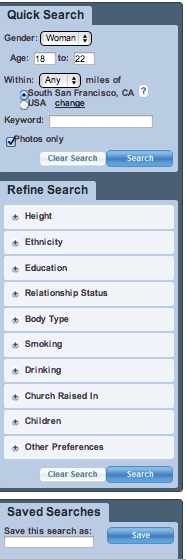
\includegraphics[width = 2in]{CM2} \\\hline
\end{tabular}
\end{table}
\subsubsection{E-Harmony}
When testing all three websites, we did not pay for any premium service. It seemed that in order to have any functional use of searching for E-harmony, a deluxe account was required. However, the basic search we used was essentially useless. The user was given no real options of advanced search, and pictures and a lot of basic information was hidden. Also, users could not refine search using a basic account. The information was displayed in an unappealing way and none of the users in this test were able to complete the experiment. 

\subsubsection{Match.com}
The Match.com search was very easy to use. Users could easily do a basic search, and many advanced options were available in the sidebar. The advanced options made refining searches very easy and quick. Also, when the text was displayed, it was displayed in a manner that was very presentable. Each match had its own box with a picture and general information. The user even had the information to hide results he/she didn't like. 

\subsubsection{ChristianMingle.com}
Christian Mingle and Match.com both had very similar side bars for searching. The many different search refinements made accomplishing the goal fairly easy. Users found the menus easy to use and understand, due to the drop down functionality of each menu. Also, users felt that since Christian Mingle used less factors to find personalities, the website has less to search through, allowing the user to find matches quicker. However, since there is less match criteria, users in the experiment felt that they could not refine searches as much as they want to. This could be because Christian Mingle users share similar interests and beliefs due to the Christian background of the site. However, there more options users felt helpful on Match.com than there were on Christian Mingle. 

\subsection{"Designers should strive to use unique and descriptive headings, and 
to use as many headings as necessary to enable users to find what 
they are looking for—it is usually better to use more rather than fewer 
headings."}

The final test of this experiment was to see if users could change their profession in their profile information. This task is fairly simple, but required users to look through the menus and bars to accomplish this task. In most cases, the test did not take very long and users could navigate menus quickly.

\subsubsection{E-Harmony.com}
E-Harmony has very few toolbar options. Users were able to change their profiles quickest on E-Harmony because there were so few menu options, and one of them was to access "my profile". If the task was to access something different on the website, the user may have had a harder time due to a lack of menu items. The user would have to scroll on the page and find links which is less efficient than an all-access toolbar.

\subsubsection{Match.com}
Match.com took advantage of a drop-down menu feature. Each toolbar option was filled with possible actions on each toolbar option. This allowed users to get what they wanted quickly. Also, if the users scrolled over the wrong toolbar, they could see that their desired option was not there, and try again without wasting clicks. 

\subsubsection{ChristianMingle.com}
Like Match.com, Christian Mingle took advantage of drop-down menus. However, once the user found their profile page, the act of editing a profile was counterintuitive. There were multiple edit buttons on the page. For some users, it took a while to figure out which edit button was appropriate to change professions. In this case, the site provided users with too many options, making the user confused and cause some errors. 

\begin{figure}
\centering

\includegraphics[width=7in]{Eharm3.png} 

\caption{Eharmony.com toolbar}
\label{Eharm3}
\end{figure}

\begin{figure}
\centering
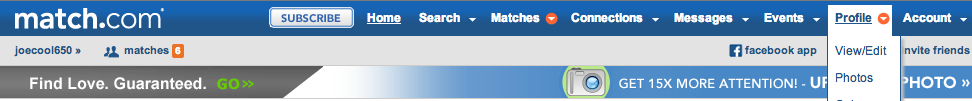
\includegraphics[width=7in]{Match3.png} 

\caption{Match.com toolbar}
\label{Match3}
\end{figure}

\begin{figure}
\centering

\includegraphics[width=7in]{CM3.png} 

\caption{ChristianMingle.com toolbar}
\label{CM3}
\end{figure}

\section{Conclusion}
Each website has its positives and its downfalls. In this section, I will summarize the performance and results of each website.

\subsection{Eharmony.com}
E-harmony scored the worst out of all the websites tested. E-harmony does a good job of highlighting features that are most used such as putting the ability to edit your profile as a main toolbar option. However, there are a lot of things on E-harmony that are unnatural to the user. The search function is very limited and frustrating. The profile questionnaire was often repetitive and users found annoyed and bored. As a result, users were not satisfied with E-harmony and said that E-harmony would not be their first choice in dating websites.

\subsection{Match.com}
Match.com scored the highest out of all three websites. Users felt very comfortable with Match.com. Online dating is already a nervous experience, so having a website that is easy to use and understand would help calm daters. All of the menus and website functions were easily accessible, and the fairly lengthy questionnaire kept users engaged leading to more accurate profiles. this was the dating website of choice for all users involved in the experiment.

\subsection{ChristianMingle.com}
In general, users were very satisfied with their experience on the site. However, the biggest complaint was that the site was too simple to be an effective tool for online dating. When answering questions, users did not appreciate the fact that they were limited by options and that there were so few questions. This led to profiles being very vague. Also, users felt that the website was confusing when it offered many options. All these options were misleading and at times, in the case of changing profession, led users astray from the actual answer.


\pagebreak
% Generate the bibliography.
%\bibliography{intro}
%\bibliographystyle{plain}

\end{document}
